\setlength{\columnsep}{3pt}
\begin{flushleft}

\begin{itemize}
	\item \textbf{Netmask} also called \textbf{subnet mask}:
	\begin{itemize}
		\item Divides one big network into small small network
		\item \textbf{Decides network bit \& host bit}
		\item The \color{blue} on bits \color{black} are \textbf{network bit} in netmask
		\item The \color{blue} on bits \color{black} decides the \textbf{netmask prefix}
		\item The \color{red} off bits \color{black} are \textbf{host bit} in netmask

	\end{itemize}	
\end{itemize}
\begin{tcolorbox}[breakable,notitle,boxrule=-0pt,colback=yellow,colframe=yellow]
	\color{black}
	\fontdimen2\font=1em
	Note: Netmask bits are always made \color{blue} on \color{black} from \textbf{left to right}.
	\fontdimen2\font=4pt
\end{tcolorbox}
\begin{figure}[h!]
	\centering
	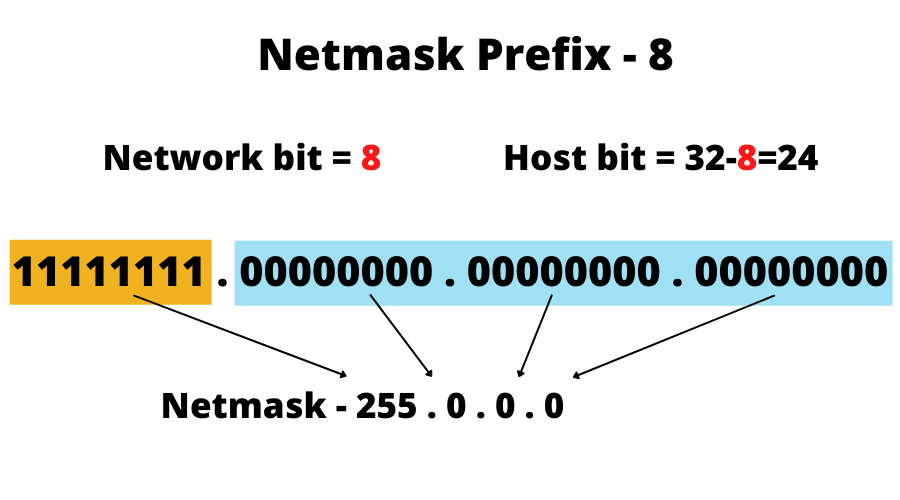
\includegraphics[scale=0.5]{content/chapter14/images/18.png}
\end{figure}
\bigskip
\begin{figure}[h!]
	\centering
	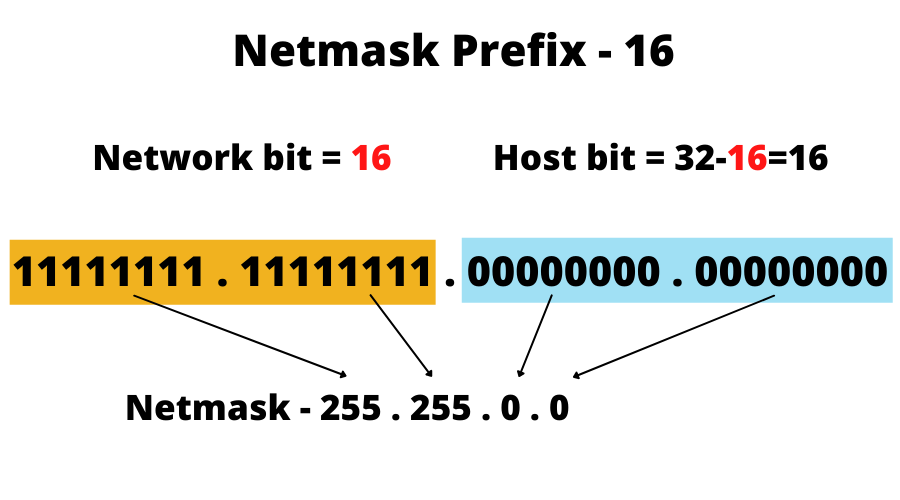
\includegraphics[scale=0.5]{content/chapter14/images/19.png}
\end{figure}
\bigskip
\begin{figure}[h!]
	\centering
	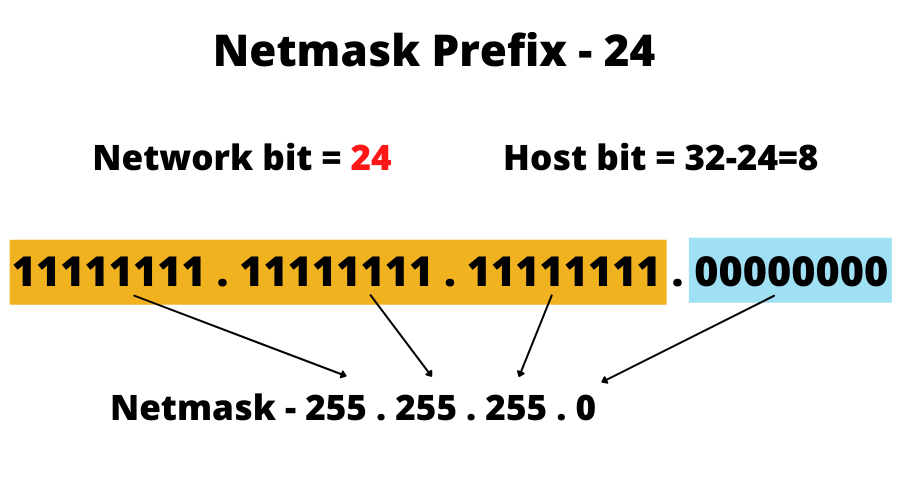
\includegraphics[scale=0.5]{content/chapter14/images/20.png}
\end{figure}
\bigskip
\begin{figure}[h!]
	\centering
	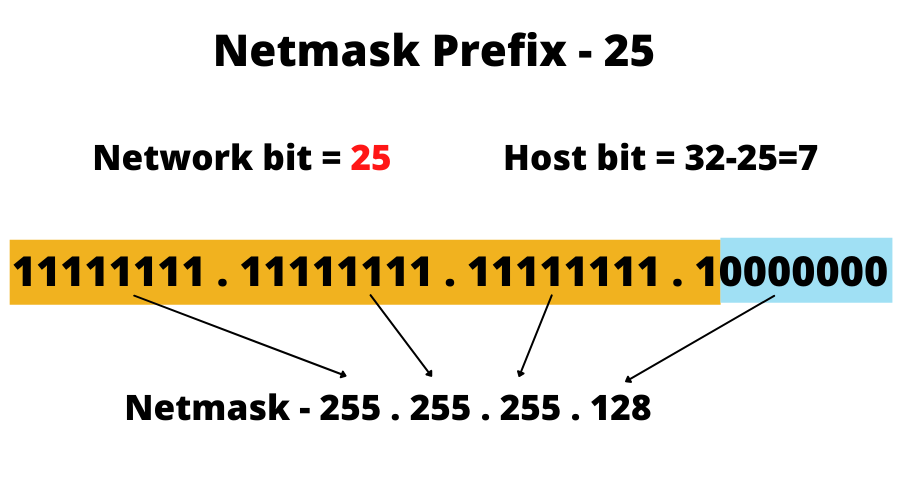
\includegraphics[scale=0.5]{content/chapter14/images/21.png}
\end{figure}
\newpage
.
\newpage

\end{flushleft}



